\documentclass[conference]{IEEEtran}
\IEEEoverridecommandlockouts
\usepackage{cite,amsmath,amssymb,graphicx,booktabs,url,xcolor}
\usepackage[T1]{fontenc}
\usepackage[utf8]{inputenc}
\def\BibTeX{{\rm B\kern-.05em{\sc i\kern-.025em b}\kern-.08em T\kern-.1667em\lower.7ex\hbox{E}\kern-.125emX}}
\begin{document}

\title{PITFALL: Catching Point-in-Time Violations in\\Multi-Table Feature Pipelines by Differential Execution}

\author{\IEEEauthorblockN{First Author, Second Author, Third Author}
\IEEEauthorblockA{ITMO University, St.\ Petersburg, Russia\\
\{author1, author2, author3\}@itmo.ru}}

\maketitle

\begin{abstract}
Features for multi-table prediction tasks are built by aggregating neighbouring
tables at a per-row seed time. Correctness requires every aggregate to respect that
seed time along every join path and for every column, including columns written to a
row \emph{after} the row appears. We show that this is violated routinely, using three
sources we did not construct: a widely used feature-engineering library called without a
cutoff-time table, as in its introductory example ($+14.8$ to $+16.3$ AUC points), the
reference code written by the authors of this paper ($+0.2$ to $+5.3$ points depending on
the task), and code generated by two language models under a neutral prompt ($53\%$ and
$35\%$ of programs that ran). We demonstrate PITFALL, which runs a feature program twice
--- on the full database and on a database physically truncated at the seed time --- and
reports any divergence. The check parses nothing, is language-agnostic, has no false
positives by construction, names the offending columns in $0.2$--$7.6$\,s, and, by
truncating one availability channel at a time, localises the leak to the table and column
it enters through. The univariate probe shipped by commercial AutoML platforms misses all
three sources at its default warning threshold and raises a false alarm on a correct
pipeline at the stricter one.
\end{abstract}

\begin{IEEEkeywords}
data leakage, point-in-time correctness, relational machine learning, AutoML,
feature engineering, LLM-generated code
\end{IEEEkeywords}

\section{Introduction}

In multi-table (relational) machine learning a prediction task is given as a table
of triples \emph{(entity, seed time, label)} over a database with foreign keys and
timestamps~\cite{relbench}. Predictive features are obtained by walking join paths
out of the entity and aggregating neighbouring rows; such features are worth on the
order of ten AUC points over the entity table alone~\cite{dbinfer}. Every aggregate
carries an obligation: it may only read facts that existed at the seed time of that
particular row.

Leakage is a documented driver of irreproducibility across applied
ML~\cite{kaufman2011,kapoor2023}, and this obligation is easy to state and easy to
violate. Truncation is \emph{per row}, so harnesses that cut the database once at the
start of the test period say nothing about individual seed times; it must hold along
\emph{every} join path, where the governing timestamp often belongs to a neighbour; and
--- the case systematically missed --- a row can carry columns written \emph{later than
the row itself}, such as a review attached to an order. Filtering by the order timestamp
admits the row and its future columns together.

Our study set out to test whether language-model agents produce leaking feature code;
the clearest evidence turned out to concern standard practice. Violations appear in
three independent sources, none constructed by us: \texttt{featuretools}~\cite{dfs}
called without a cutoff-time table, the form of its introductory
example~\cite{ftdocs}; the reference implementation written by the authors of this
paper, found by our own checker; and single-shot generations from two language models
under a prompt that never mentions leakage.

Existing safeguards do not cover this case. Commercial AutoML platforms (DataRobot,
H2O Driverless AI, SageMaker Data Wrangler) ship the same univariate probe --- flag a
feature whose single-feature AUC exceeds a threshold~\cite{datarobot,h2o}. Rule-based
checkers such as \texttt{leakr}~\cite{leakr2025} enumerate a fixed list of patterns.
Static analyzers for notebooks~\cite{yang2022} and pipeline instrumentation such as
\texttt{mlinspect}~\cite{mlinspect} target preprocessing order and train/test
contamination, not temporal leakage. Asking a language model
directly performs poorly: low-shot prompting reaches $0.19$ precision at $0.52$ recall,
against $0.86/0.70$ for a trained classifier~\cite{peerj2025}.

\textbf{Contributions.} (i) \emph{Differential execution} as a correctness check for
feature programs: sound, one-sided, independent of language and of any understanding
of the code, with leak localisation by per-channel truncation. (ii) Evidence from three
independent sources that point-in-time violation is routine. (iii) An execution-verified
measurement of the rate at which two language models produce temporally incorrect
feature code for a multi-table task, decomposed by task construction and prompt guard
strength. (iv) A working system and a four-scene demonstration in which the checker
fires where the industrial probe is silent, stays silent where the code is correct, and
localises and patches the leak.

\section{Point-in-Time Correctness}

\subsection{Definition}
Let $D$ be a database, $t$ a seed time and $\varphi$ a feature program. Each row $r$ has
a row timestamp $\mathrm{time}(r)$; a column $c$ of $r$ may in addition have its own
availability timestamp $\mathrm{avail}_c(r)\ge\mathrm{time}(r)$. Write $D|_t$ for the
database in which rows with $\mathrm{time}(r)>t$ are removed and values with
$\mathrm{avail}_c(r)>t$ are replaced by NULL. Then $\varphi$ is \emph{point-in-time
correct at $t$} iff
\begin{equation}
\varphi(D,t)=\varphi(D|_t,t).
\label{eq:pit}
\end{equation}
For a cutoff shift $\delta\ge 0$ we write $I(\delta)$ for the AUC of a \emph{fixed}
learner $A$ trained and evaluated on features computed with cutoff $t+\delta$, minus its
AUC at $\delta=0$. Fixing $A$ matters: in one agent trajectory~\cite{relagent} we
examined, swapping the boosting implementation on a bit-identical feature set moved AUC by
$11.5$ points, the order of the effect measured here.

\subsection{Availability relation}
Equation~(\ref{eq:pit}) generalises by replacing the time predicate with an
\emph{availability relation} $R(r,e,t)$, true when row $r$ may be read when predicting
for entity $e$ at time $t$; co-emission and group leakage are other masks over the same
machinery. Availability is defined \emph{per column}: in our data \texttt{review\_score} becomes available at
\texttt{review\_creation\_date}, a median of 10 days (max 147) after the order row it is
attached to. Some columns admit \emph{no} availability timestamp --- a mutable status
field kept without history. For such a column the truncated database is
indistinguishable from the full one and no execution-based check can decide it. We
exclude one such column (\texttt{order\_status}) from all conditions rather than report
an undecidable case as clean.

\subsection{Why univariate probes are the wrong instrument}
If a leaked signal of fixed total strength is spread over $d$ aggregate features, its
visibility to any single-feature statistic shrinks with $d$ while its effect on a
multivariate model does not; with enough aggregates a leak of arbitrary strength stays
below any univariate threshold. Fig.~\ref{fig:blind} shows this empirically; when
leakage concentrates in one feature the probe does see it, as on one of our three tasks.

\subsection{Differential execution and localisation}
The check follows from~(\ref{eq:pit}): run $\varphi$ twice and compare.
\begin{center}\small\ttfamily
full\ \ = program(db, t, entities)\\
trunc = program(db.truncate(t), t, entities)\\
verdict = (full != trunc)
\end{center}
A divergence is a \emph{proof} of violation: the same program, given strictly less
information, produced a different answer --- whether through an aggregate, a join, or a
statistic fitted on the full table. There are no false positives by construction. The
guarantee is one-sided --- a violation that does not manifest at the tested seed time is
not observed --- and the program must be deterministic and re-runnable.

The same primitive localises the leak. The database has a finite set of
\emph{availability channels}: ``rows of table $T$ appearing after $t$'' and ``values of
column $c$ becoming known after $t$''. Truncating one channel at a time and re-running
$\varphi$ names the channels on which the output changes and the output columns each
affects; the minimal patch --- truncate the input on exactly those channels --- is then
re-checked. This costs one run per channel (seven in our database) and still reads no
code.

\section{System}

\begin{figure}[t]\centering
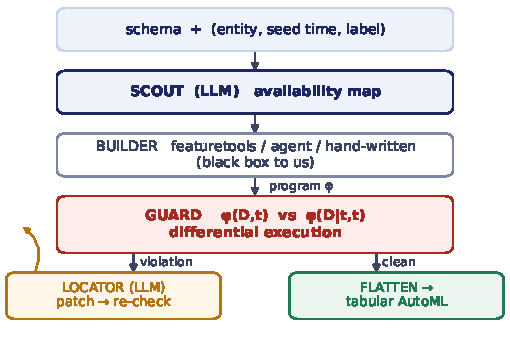
\includegraphics[width=.92\columnwidth]{fig/fig1_arch.pdf}
\caption{PITFALL sits between any feature builder and any tabular AutoML. \textsc{Guard}
and \textsc{Locator} are deterministic; the availability map consumed by \textsc{Scout}
is hand-written in the current release and may be proposed by an LLM.}
\label{fig:arch}
\end{figure}

Fig.~\ref{fig:arch} shows the pipeline. \textsc{Scout} holds the availability map ---
which column governs the availability of which field, and which fields have none. In the
current release the map is a small hand-written declaration (row-time column per table,
value-time column per late-written field); an LLM may propose it from the schema --- a
schema question whose answer is independently checkable, unlike ``is there leakage
here''~\cite{peerj2025}. \textsc{Builder}
is anything that emits a feature program: a library, an agent, a human. \textsc{Guard}
performs the differential check and returns a verdict, the list of diverging columns and
the number of diverging cells. On a violation, \textsc{Locator} runs the per-channel
truncation, reports which channel feeds which output column, applies the minimal input
patch and re-checks. Clean programs are flattened into a single table and handed to an
unmodified tabular AutoML system such as AutoGluon~\cite{autogluon}. The core is about
170 lines of Python over pandas and numpy, with no dependency on the builder's language.

\textbf{Validating the checker.} On six reference programs with known verdicts (correct;
leak in the entity's own history; leak only through a join; both; no cutoff; and our
original ``correct'' code, see below) at three seed times, the checker was right on
18 of 18 combinations. As a negative control we set the seed time to the maximum
timestamp in the database, where every aggregation is correct by construction and the
expected result is zero alerts. The first run of that control was not zero: two null
outputs were compared as unequal, so programs that returned nothing looked like
violations. The control ran before the main experiment, as pre-registered; re-auditing
the 23 verdicts issued until then found one false.

\section{Evidence}

\textbf{Setup.} Olist~\cite{olist}, a public Brazilian marketplace database: 7 tables,
112{,}650 order line items, September 2016 to October 2018. Three tasks in
RelBench~\cite{relbench,relbench2} form --- seller activity (A), seller review quality
(B), product demand (C) --- three seed times (January, April, July 2018), 90-day horizon,
training on all earlier seed times; 750--870 sellers and 4{,}500--5{,}800 products per
seed time. One LightGBM configuration with a fixed seed everywhere. Two cores, no GPU.

\subsection{The cost of a shifted cutoff}
$I(\delta)$ grows monotonically over $\delta\in[0,90]$ days on tasks A and B at all
three seed times: a one-month error already costs $5.8$--$11.5$ points, and removing the
cutoff entirely yields $+12.3$ to $+27.0$ (A) and $+5.8$ to $+18.0$ (B). For scale: on
flat tabular data the mean loss from picking the validation winner among 63 pipelines
(16 datasets, 3 seeds) is $0.38$ points. On task C we control the cutoff
separately for the entity's own history and for aggregates reached \emph{through a join}
to the seller: leaking only through the join costs $+3.0$ to $+5.1$ points and, as
Section~\ref{sec:blind} shows, is invisible to the probe.

\begin{table}[t]
\caption{Sources of point-in-time violation. Rows 1, 2 and 5 were not constructed by
us; row 4 is a controlled regime. ``Probe'' is the maximum single-feature AUC on the
leaking features; DataRobot warns at $0.85$, H2O Driverless AI at $0.80$.}
\label{tab:sources}
\centering\scriptsize
\setlength{\tabcolsep}{2.4pt}
\begin{tabular}{@{}lccc@{}}
\toprule
Source & Inflation, pp & Probe & at 0.85 / 0.80 \\
\midrule
\texttt{featuretools}, no cutoff table & $+14.8\ldots+16.3$ & $0.76$--$0.83$ & silent / warns 2/3 \\
Our reference code, task B & $+3.1\ldots+5.3$ & $0.62$--$0.69$ & silent / silent \\
\quad same defect, tasks A and C & $-0.1\ldots+1.0$ & $0.71$--$0.86$ & silent$^\dagger$ \\
Leak through a join path only & $+3.0\ldots+5.1$ & unchanged & silent / silent \\
LLM code, neutral prompt & median $+0.1$ & --- & $53\%$ / $35\%$ violate \\
\bottomrule
\end{tabular}\\[2pt]
{\scriptsize $^\dagger$On task A the probe crosses both thresholds on the \emph{correct}
pipeline too (Section~\ref{sec:blind}).}
\end{table}

\subsection{Violation is routine}
Table~\ref{tab:sources} collects the sources.

\emph{A library, called as in its introductory example.} \texttt{featuretools} 1.31.0
with \texttt{ft.dfs} and no cutoff-time table inflates AUC by $14.8$, $16.3$ and $15.6$
points on the three seed times of task C. The library supports cutoff times; it does not
signal that they are needed. An independently written harness reproduces the probe values
to three decimals ($0.834/0.809/0.759$).

\emph{Expert code, written by us.} Our reference implementation filtered history by
order time and then took all columns of the admitted rows. Two of those columns have
their own, later timestamps: the review score and the delivery outcome. Across the
three seed times, $5.0\%$, $5.0\%$ and $2.0\%$ of orders placed before the seed time
carry a review written after it. The checker flagged exactly four columns
(\texttt{review\_score\_mean}, \texttt{review\_score\_min}, \texttt{late\_mean},
\texttt{delay\_days\_mean}) and no others. Cost: $+3.09$, $+5.26$, $+3.78$ points on
task B, but only $+0.16$ to $+0.31$ on A and $-0.10$ to $+0.98$ on C.

\emph{Published expert SQL.} In the hand-written feature SQL of the RelBench user
study~\cite{relbench} (15 files, 172 joins), a manual audit found two genuine
violations, roughly $1\%$ of joins; a syntactic scanner raised eight candidates of which
six were false. This audit was static (the database was not reachable from our
environment) and we report it as such.

\begin{figure}[t]\centering
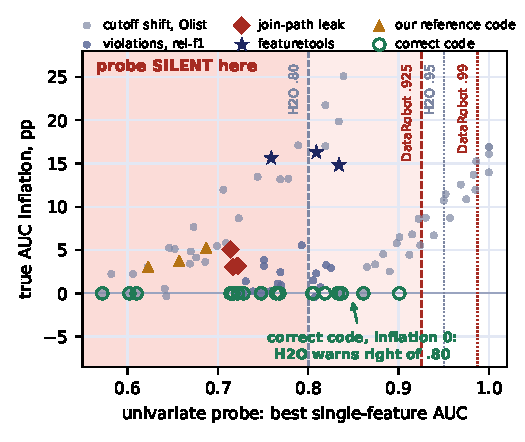
\includegraphics[width=.96\columnwidth]{fig/fig4_blind.pdf}
\caption{Probe value against true inflation. Every point left of $0.85$ is a violation
the DataRobot probe does not report, including all three sources of
Table~\ref{tab:sources}; the H2O threshold of $0.80$ catches two of three
\texttt{featuretools} points and none of the others.}
\label{fig:blind}
\end{figure}

\subsection{The deployed test does not see it}\label{sec:blind}
Fig.~\ref{fig:blind} plots the probe value against true inflation. The cleanest case is
leakage through a join: the probe returns $0.714/0.722/0.717$ under a correct cutoff and
\emph{the same} $0.714/0.722/0.717$ under leakage, while the model gains $3.0$--$5.1$
points. On task B no condition --- including the total absence of a cutoff, worth
$+18.0$ points --- reaches $0.80$. The failure runs in both directions: on task A the
\emph{correct} pipeline scores $0.837/0.861/0.833$, above $0.80$ at every seed time and
above $0.85$ at one, because recency is legitimately the strongest predictor of churn.
Lowering the threshold trades misses for false alarms; no threshold separates the two.

\subsection{Generated feature code}
We asked two models --- \texttt{deepseek-v4-flash} and
\texttt{bytedance-seed/seed-2.0-code} --- for a Python function computing features for
task C, giving the schema, the training table with the seed-time column named, and
nothing else: the words ``leakage'' and ``point-in-time'' do not appear. Each generation
is single-shot with a clean context at temperature $0.7$; verdicts come from the checker;
five of the flagged programs were additionally read by hand and confirmed. Of 40
generations per model, 30 and 17 ran (the rest failed to execute and are excluded, which
may bias the rate in either direction). Of those, $53.3\%$ [$36.1$, $69.8$] and $35.3\%$
[$17.3$, $58.7$] were incorrect. The failure is the same in every case examined: the
model filters the entity's own history by the primary event timestamp and does not
account for the later timestamp of the joined entity. We make no claim about model
capability in general.

Two follow-ups locate the effect. \emph{Task construction} decides it: on a second task
with a single seed time per entity, only the entity's own history and no secondary time
axis, both models produce $0$ violations in 24 and 28 running programs. \emph{Prompt
guards help partially} (30--40 generations per cell, 9--30 running): moving from a
neutral prompt to a general reminder to a per-aggregate requirement takes the pooled rate
from $46.8\%$ [$33$, $61$] to $41.2\%$ [$26$, $58$] to $14.6\%$ [$7$, $28$] --- monotone,
but not zero.

\subsection{The cost of a violation is not implied by the violation}
The same defect --- the same secondary time axis, the same code --- costs $0.16$--$0.31$
points on task A, $-0.10$--$0.98$ on C and $3.09$--$5.26$ on B; among model-generated
programs the median inflation is $0.11$ points (range $-2.2$ to $+2.0$). Cost depends on
how many features are touched and how much the target leans on them, neither visible from
the fact of the violation. Correctness therefore has to be tested separately from the
quality metric, which an execution-based checker does and a metric-based heuristic cannot.

\section{Demonstration}

\begin{figure}[t]\centering

\includegraphics[width=.95\columnwidth]{fig/fig5_demo.png}
\caption{Scene 4 of the demonstration page: \textsc{Locator} names the availability
channel behind each diverging column and re-checks the patched program.}
\label{fig:demo}
\end{figure}

The demonstration runs offline on a laptop in about two minutes
(\texttt{python3 demo.py}), prints per scene a verdict, the diverging columns, the probe
value at both thresholds and the true inflation, and renders the same results as a
self-contained page (Fig.~\ref{fig:demo}). Attendees can edit a scene's feature
function and re-run the check.

\textbf{Scene 1 --- library defaults.} \texttt{ft.dfs} without a cutoff-time table.
Verdict \textsc{violation} in $7$\,s, 11 diverging columns, 19{,}334 cells; probe
$0.809$ (silent at $0.85$, warns at $0.80$); inflation $+16.3$ points.

\textbf{Scene 2 --- our own code.} Verdict \textsc{violation} in $0.2$\,s, naming
exactly the four review and delivery aggregates; probe $0.687$, silent at both
thresholds; $+5.3$ points. This code was written and read by the authors of the checker.

\textbf{Scene 3 --- the fix.} The same program with the availability relation fixed and
nothing else changed. Verdict \textsc{clean}, outputs identical, inflation $0.00$ at all
three seed times: the negative control for the first two scenes.

\textbf{Scene 4 --- localisation.} \textsc{Locator} truncates the seven availability
channels one at a time. For Scene 2 it attributes the two review aggregates to
\texttt{review\_score} becoming known after $t$ and the two delivery aggregates to the
delivery date; for Scene 1 it attributes all eleven columns to \texttt{items} rows
appearing after $t$. In both cases the minimal input patch re-checks \textsc{clean}.

\section{Limitations}

\emph{(i) One-sided.} The check proves violation, never correctness, and only with
respect to the observed database and the chosen mask. \emph{(ii) Undecidable
columns.} Mutable fields kept without history admit no availability timestamp and cannot
be checked by execution at all. \emph{(iii) Dependence on the availability map.} If the
map assigns the wrong timestamp, the wrong thing is checked. \emph{(iv) Scope of
measurement.} One database, three tasks, three seed times; two models at one price tier;
rates on generated code describe practice under specific prompts at a point in time.
\emph{(v) Final-program metric undercounts.} An agent's validation-driven selection can
discard a leaking intermediate trial, as we observed once; checking only the final
artifact understates the rate.

\section{Conclusion}

Point-in-time correctness in multi-table feature pipelines is violated routinely, and the
univariate probe deployed to catch it is silent in exactly the regimes that matter.
Differential execution decides the question in seconds without parsing anything,
localises the leak by the same primitive, and states the class it cannot decide.

\section*{Data and Ethics}
All experiments use the public Olist dataset (Kaggle, CC BY-NC-SA 4.0), anonymised by
its publisher; no human subjects were involved. Language-model outputs were used only as
objects of measurement, unedited, and are released with the code.

\section*{Availability}
Code, data and all reported numbers:
\url{https://github.com/stas1f1/pitfall}.

\begin{thebibliography}{99}\footnotesize
\bibitem{kaufman2011} S.~Kaufman, S.~Rosset, and C.~Perlich, ``Leakage in data mining: formulation, detection, and avoidance,'' in \emph{Proc. KDD}, 2011.
\bibitem{kapoor2023} S.~Kapoor and A.~Narayanan, ``Leakage and the reproducibility crisis in machine-learning-based science,'' \emph{Patterns}, vol.~4, no.~9, 2023.
\bibitem{yang2022} C.~Yang \emph{et al.}, ``Data leakage in notebooks: static detection and better processes,'' in \emph{Proc. ASE}, 2022.
\bibitem{mlinspect} S.~Grafberger, S.~Guha, J.~Stoyanovich, and S.~Schelter, ``mlinspect: a data distribution debugger for machine learning pipelines,'' in \emph{Proc. SIGMOD}, 2021.
\bibitem{peerj2025} N.~Alturayeif and J.~Hassine, ``Data leakage detection in machine learning code: transfer learning, active learning, or low-shot prompting?'' \emph{PeerJ Computer Science}, 11:e2730, 2025.
\bibitem{leakr2025} C.~Isabella, ``leakr: data leakage detection,'' CRAN package, 2025.
\bibitem{datarobot} DataRobot, ``Target leakage,'' product documentation, \url{https://docs.datarobot.com}, accessed Aug.\ 2026.
\bibitem{h2o} H2O.ai, ``Driverless AI: leakage detection,'' product documentation, \url{https://docs.h2o.ai}, accessed Aug.\ 2026.
\bibitem{relbench} J.~Robinson \emph{et al.}, ``RelBench: a benchmark for deep learning on relational databases,'' in \emph{NeurIPS Datasets and Benchmarks}, 2024.
\bibitem{relbench2} J.~Gu, R.~Ranjan, C.~Kanatsoulis \emph{et al.}, ``RelBench v2: a large-scale benchmark and relational data repository,'' in \emph{ICLR Workshop on Foundation Models for Tabular and Structured Data (DATA-FM)}, 2026.
\bibitem{dbinfer} M.~Wang \emph{et al.}, ``4DBInfer: a 4D benchmarking toolbox for graph-centric predictive modeling on relational DBs,'' in \emph{NeurIPS Datasets and Benchmarks}, 2024.
\bibitem{relagent} ``RelAgent: agentic feature engineering for relational data,'' arXiv preprint arXiv:2605.07840, 2026. (Preprint; not peer reviewed.)
\bibitem{dfs} J.~M.~Kanter and K.~Veeramachaneni, ``Deep feature synthesis: towards automating data science endeavors,'' in \emph{Proc. DSAA}, 2015.
\bibitem{ftdocs} Featuretools, ``Handling time,'' documentation for v1.31, \url{https://featuretools.alteryx.com}, accessed Aug.\ 2026.
\bibitem{autogluon} N.~Erickson \emph{et al.}, ``AutoGluon-Tabular: robust and accurate AutoML for structured data,'' arXiv preprint arXiv:2003.06505, 2020.
\bibitem{olist} Olist, ``Brazilian e-commerce public dataset,'' Kaggle, 2018.
\end{thebibliography}

\end{document}
